
\section*{O pensamento musical na Idade
Media}\label{o-pensamento-musical-na-idade-media}

O concepto ---e a expresión--- de «Idade Media» foi creado polos
humanistas europeos do Renacemento para referirse ao período que
separaba a Antigüedad clásica da Modernidade que eles mesmos
representaban. A súa admiración extrema pola arte e o pensamento dos
\emph{antigos} gregos e romanos e o seu desexo de recuperalos nunha
idade \emph{moderna} leváronos ao desprezo por toda a etapa
\emph{intermedia} entre ambos mundos, ignorando ou rexeitando toda
evolución artística, científica e filosófica desa época. Sería moito
máis tarde, xa no século XIX, cando os artistas e pensadores de Europa
rescatarían esa «Idade Media» e farían dela un período mítico de ideais
``caballerescos'', amorosos e relixiosos, nun enfoque igualmente tan
erróneo como o dos seus predecesores.


En realidade, o período que seguimos denominando \emph{medieval} é unha
continuación directa da época clásica, sen presentar unha ruptura clara;
mais nos aproximadamente mil anos que atribuímos a esa época sucedéronse
numerosas formulacións novas en canto á arte ou ao pensamento, e tamén
en canto ao pensamento musical. As ideas e o pensamento musical medieval
foi en gran parte unha prolongación do antigo, onde as ideas principais
quedaron «fosilizadas» durante séculos, houbo tamén enfoques novos desas
mesmas ideas; e, o que é máis importante, formulacións absolutamente
novas, en especial no que respecta á música práctica, tanto nos seus
aspectos técnicos e sistemáticos como na pedagoxía musical; e, de
maneira aínda máis relevante, na escritura musical.

\begin{figure}[h]
\centering
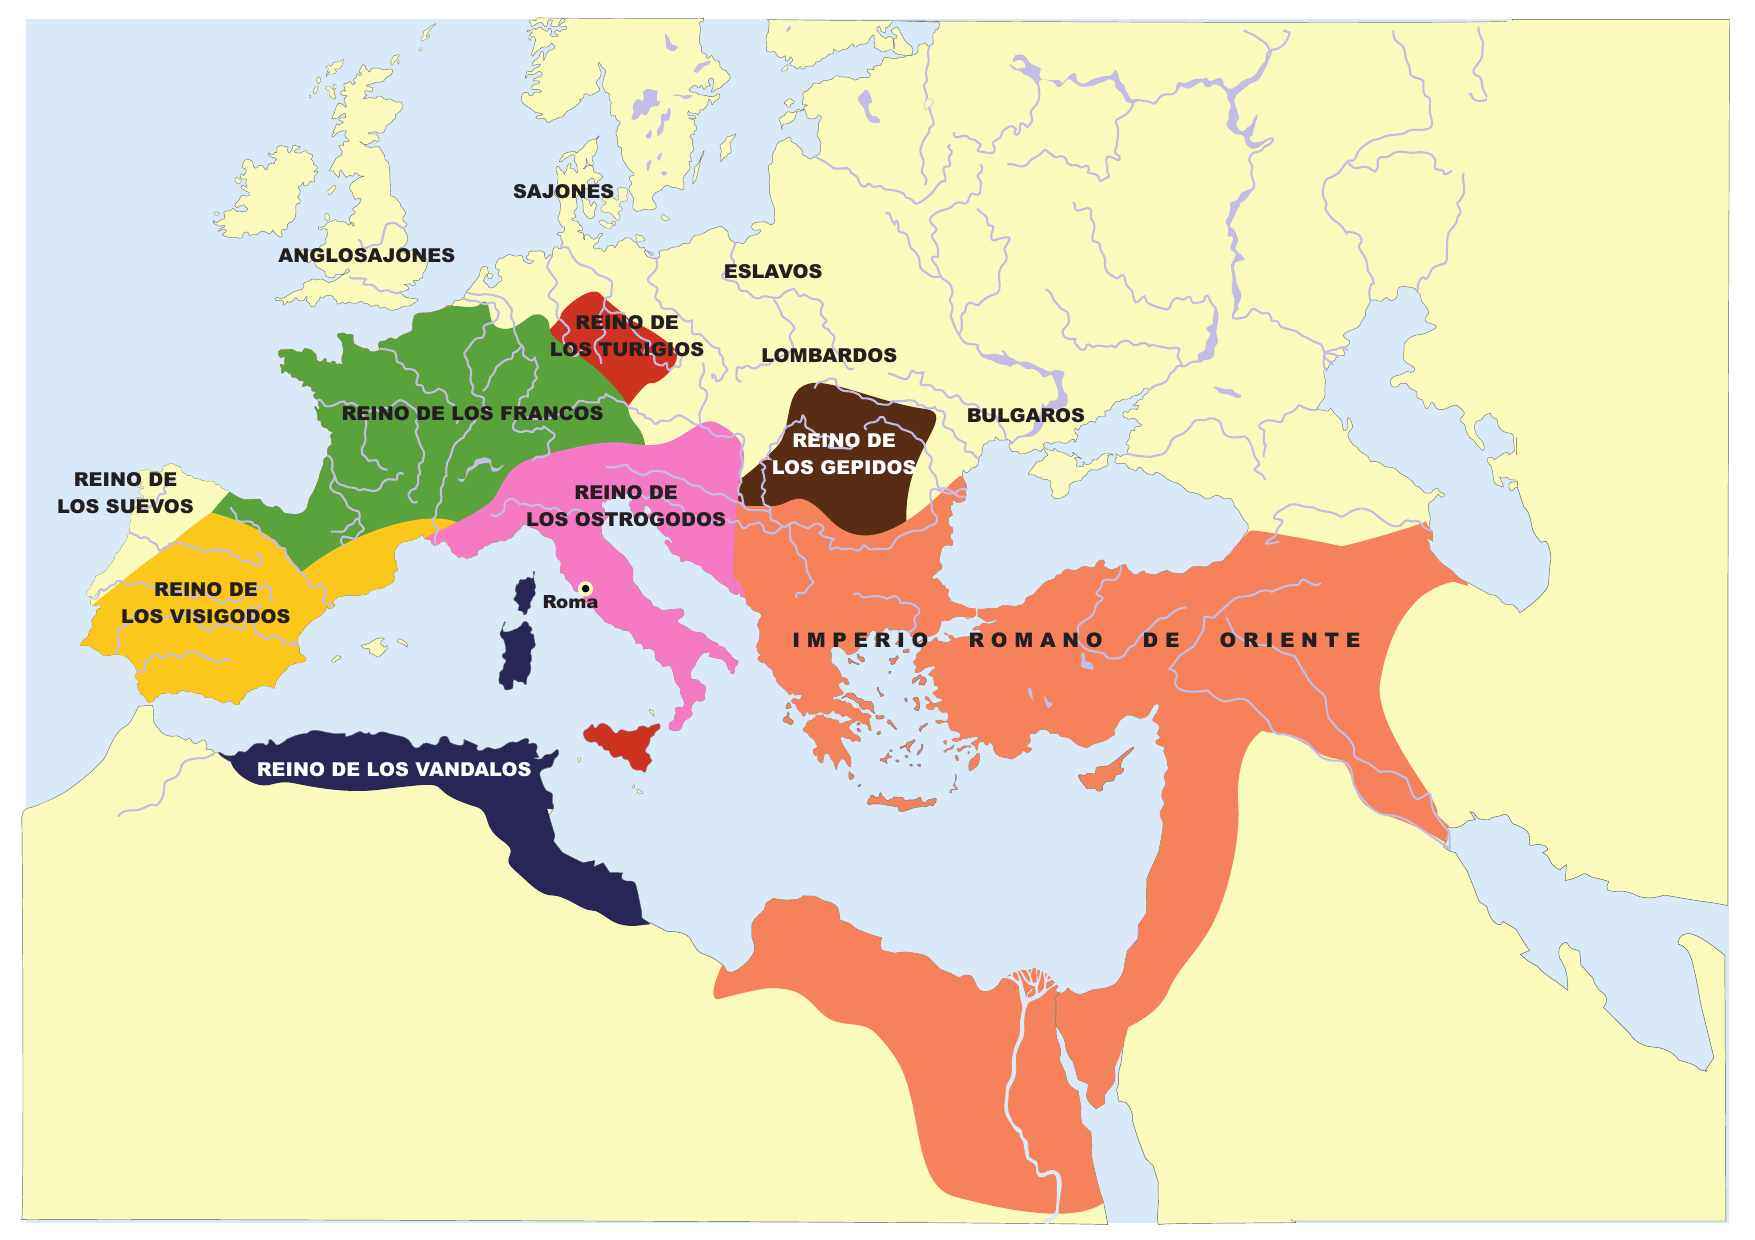
\includegraphics[scale=0.55]{ud-03/mapa_reinos_germanicos.png}
\caption{División política do Mediterráneo c.a 500.\\
(Fonte: Banco de recursos pntic - mec)}
\label{fig:mapa-xermanicos}
\end{figure}

\begin{multicols}{2}

\subsection*{Contexto histórico}\label{o-contexto-historico}

O comezo da Idade Media adoita situarse cara o ano 476 d.C, coincidindo
coa caída do imperio romano de occidente, se ben en realidade isto foi
só a constatación «oficial» de algo que levaba sucedendo desde case dous
séculos antes: a ruptura entre o Oriente \emph{romano} ---que
denominamos \emph{bizantino}--- e o Occidente \emph{xermanizado}, no que
as estruturas do Imperio desapareceran case na súa totalidade.

O período fundamental neste proceso de cambio foi o século IV, en
especial durante os mandatos dos emperadores Constantino, ao comezo do
século, e Teodosio, ao final. Ambos tomaron decisións que influirían
decisivamente no futuro do Imperio: no 313, Constantino decretou o
\emph{Edicto de Milán}, polo que se permitía a liberdade relixiosa e
finalizaban as persecucións; ata entón Roma fora bastante tolerante en
materia relixiosa, pero o culto ao emperador e a certos deuses era
obrigatorio, o cal afectaba principalmente as relixións monoteístas. O
edicto\footnote{As consecuencias do Edicto de Milán foron máis aló do
  recoñecemento da liberdade relixiosa para os cristiáns. Esta
  proclamación conlevou cambios profundos dentro do Imperio romano, así
  como a expansión da Igrexa e o aumento paulatino do seu poder. O
  contido literal do edicto non outorgaba ao cristianismo unha
  importancia especial, xa que se refire á liberdade de cada cidadán de
  practicar a relixión que elixise. O edicto significou a devolución dos
  lugares de culto aos cristiáns, así como das propiedades que foran
  confiscadas polos romanos e vendidas a particulares. Isto deu ao
  cristianismo un maior recoñecemento legal, ata poñerse ao mesmo nivel
  que a relixión romana. Algúns anos máis tarde, converteuse na relixión
  oficial do Imperio e dos seus exércitos. Co Edicto de Milán, o
  paganismo deixou ser a relixión oficial do Imperio romano. A partir
  dese momento, os cristiáns tiveron os mesmos dereitos que o resto dos
  cidadáns.} foi especialmente beneficioso para o cristianismo, que por
entón comezaba a estenderse entre as clases altas do Imperio; a partir
deste edicto, as conversións entre a aristocracia imperial foron
numerosas, converténdose \emph{de feito} na relixión do Imperio; isto
foi ratificado no ano 392 por Teodosio, que proclamou o cristianismo
como relixión \emph{oficial}.

Por outra banda, Constantino mandou edificar unha cidade sobre o
emprazamento da antiga Bizancio, xunto ao Bósforo, para convertela en
capital do Imperio. Isto era a proba definitiva da decadencia da cidade
de Roma, que desde tempo atrás deixara de ser sede imperial. O traslado
da capitalidade á nova Constantinopla supoñía un reforzo da zona
oriental ---grega--- do Imperio, en prexuízo da occidental latina.\\
O deterioro desta última agravouse coa decisión de Teodosio, ao seu
pasamento, de dividir o control do Imperio entre os seus dous fillos:
Arcadio, o maior, gobernaría como emperador desde Constantinopla e
Honorio, sometido ao seu irmán, gobernaría Occidente, primeiro desde
Milán e despois desde Ravena. Esta situación manteríase oficialmente ata
o 476, a pesares de que Occidente experimentaría unha progresiva
\emph{xermanización}, co asentamento de varios pobos (principalmente
visigodos, ostrogodos e francos) que acabaría coa súa fragmentación en
diversos reinos, teoricamente sometidos ao emperador romano de Oriente.
Esta situación complicarase a partir do século VII coa expansión do
Islam despois da morte de Mahoma: o espazo do antigo Imperio Romano
dividirase así en tres zonas diferenciadas no terreo relixioso, político
e cultural: o Imperio, de cultura grega e relixión cristiá ortodoxa; o
mundo árabe musulmán; e o Occidente xermano-latino e católico.

Os primeiros séculos da Idade Media ---coñecidos habitualmente como
«Alta Idade Media»--- caracterízanse en Occidente, ademais de por esta
fragmentación, por unha progresiva \emph{ruralización}, co abandono das
cidades e a desaparición das súas institucións. A nobreza,
principalmente guerreira á maneira xermánica, instálase no medio rural
en castelos e fortalezas illadas. A única institución do Imperio que
permanece forte é a Igrexa, cada vez máis ruralizada tamén, cos
mosteiros como focos importantes. A actividade cultural será exclusiva
destes mosteiros, que aportan unha influencia notable do relixioso sobre
a cultura da época.
Esta situación mantense practicamente ata o século XII, con momentos
relevantes de «renacemento» cultural, como a corte de Carlomagno en
Aquisgrán entre os séculos VIII e IX ou o florecemento do movemento trovadoresco en
\href{https://es.wikipedia.org/wiki/Aquitania}{Aquitania} no século XII.
A partir do século XI, con todo, comeza unha nova etapa, a «Baixa Idade
Media», cunha reurbanización progresiva: as institucións culturais
principais xa non serán só os mosteiros, senón as catedrais e, de modo
moi especial, as universidades, a partir da fundación da Universidade de
Bolonia no 1088; os nobres, especialmente os monarcas, tamén se
instalarán en palacios urbanos. Isto provocará un importante avance
cultural que conducirá en definitiva ao Renacemento.

\subsection*{O pensamento musical}\label{o-pensamento-musical}

\subsubsection*{Alta Idade Media}\label{alta-idade-media}

Durante a Alta Idade Media non se produce unha ruptura importante coas
ideas musicais anteriores, salvo a progresiva «cristianización» das súas
teorías. Mantéñense así a teoría da \emph{harmonía das esferas} (coa
única modificación ---importante--- da intervención divina) e a teoría
do \emph{ethos}, que se relacionará agora cos distintos modos da música
medieval, especialmente a relixiosa. O principal «responsable» desta
continuidade é o filósofo romano \textbf{Severino Boecio}, que crea o
tratado \emph{De institutione musica}, moi citado ---e copiado---
durante toda a Idade Media e moito despois.

A primeira cuestión estritamente medieval, que aparece xa no século IV,
é o debate sobre a conveniencia ou non do uso da música nas cerimonias
relixiosas: a postura dominante é contraria, en principio, dada a
sensualidade da música. Así, en palabras do escritor cristián Lactancio:

\begin{quote}
\small{
O pracer dos oídos orixínase na suavidade das voces e dos cantos; e
inclina ao \emph{vicio} tanto como o dos ollos, como dixemos.}\footnote{Lucio
  Cecilio Firmiano Lactancio (c. 245 -c. 325) foi un escritor latino e
  apoloxista
  cristián do norte de África, discípulo do maestro africano de
  retórica
  \href{https://es.wikipedia.org/wiki/Arnobio_de_Sicca}{Arnobio}.}
\end{quote}

Fronte a esta postura, outros, como
Ambrosio de Milán ou Agustín de Hipona, defenden o uso da música:

\begin{quote}
\small{A quen elevar este canto senón a Deus?}
\end{quote}

Outro debate central durante toda a Idade Media, herdanza tamén do mundo
antigo, é a oposición entre música teórica e música práctica, definida
na época medieval cos termos de músico e \emph{cantor}. O «músico» é o
teórico que coñece os fundamentos da ciencia musical, especialmente a
súa base matemática; o «cantor», pola súa banda, é quen leva á práctica
a música, como un oficio. O prestixio da ciencia e o desprezo polo
traballo manual que caracteriza boa parte do pensamento medieval, fan
que se sitúe tamén por encima o papel do músico fronte ao do cantor; a
música, por outra banda, será parte dos estudos superiores de ciencias,
o \emph{quadrivium}, xunto coa aritmética, a xeometría e a astronomía.

Por último, hai que ter en conta que o sistema de escritura musical que
se utilizou desde o século IV a.C deixa paulatinamente de usarse a
partir do século II d.C, o que leva a desenvolver na Alta Idade Media a
idea de que a música reside só na memoria, e é por tanto un exemplo da
fugacidade. En palabras de
\href{https://es.wikipedia.org/wiki/Isidoro_de_Sevilla}{Isidoro de
Sevilla}:

\begin{quote}
\small{
Se os sons non se reteñen na memoria humana, perecen, xa que non poden
escribirse.
}
\end{quote}

\subsubsection*{Baixa Idade Media}\label{baixa-idade-media}

As teorías indicadas séguense mantendo sen apenas modificación durante
toda a Idade Media, case sempre repetindo literalmente as palabras de
Boecio. Con todo, a partir do século IX comeza unha nova liña nas
formulacións musicais que terá un peso decisivo nos últimos séculos
medievais: trátase da importancia dada á música práctica, tanto nos seus
aspectos máis técnicos (sistema musical) como nos didácticos, entre os
que se incluiría o interese cada vez maior por desenvolver unha notación
musical adecuada.

No primeiro aspecto hai que partir dos tratados anónimos \emph{Musica
enchiriadis} e \emph{Scolica enchiriadis}, ambos do século IX, que xunto
cos libros de \href{https://es.wikipedia.org/wiki/Hucbaldo}{Hucbaldo}
inauguran toda unha serie de tratados musicais que chegará ata o mesmo
Renacemento. En todos estes tratados inclúense habitualmente as teorías
antigas sobre a música, pero a súa formulación central é sempre a
sistematización da música da súa época, clasificada en modos aos que se
adoita atribuír un \emph{ethos} determinado. Tratan tamén aspectos
referentes á interpretación musical, como o uso da ornamentación e da
polifonía improvisada.

Na mesma liña, e cunhas características pedagóxicas importantes, hai que
situar a obra de \textbf{Guido d'Arezzo} (século XI), que desenvolveu un
sistema didáctico baseado en
\href{https://es.wikipedia.org/wiki/Mano_guidoniana}{hexacordos} en que
cada nota estaba asociada a unha sílaba mnemotécnica (a base do actual
solfexo), así como un sistema organizado de notación musical que se
impuxo rapidamente e que evolucionou despois ata o sistema actual.

Por último, o debate sobre a conveniencia da música que se orixinou no
século IV, continuará na Baixa Idade Media asociado agora á polifonía e
os seus diferentes estilos, considerados en ocasións como inadecuados
para o seu uso litúrxico.

\end{multicols}

\begin{ejercicio}[Pensamento musical Idade Media]
\begin{enumerate}[1.-]
 \item
 Resume brevemente as características do pensamento musical na Alta Idade Media.
 \vspace*{6.60cm}
 \item
 Indica de xeito resumido as características do pensar musical na Baixa Idade Media.
 \vspace*{6.6cm}
\end{enumerate}


% ESPACIO PARA REDACTAR O COMENTARIO DA AUDICIÓN
%
%\small{}
%\small{Trátase dunha forma vocal menor, de estrutura ternaria; segundo o ámbito e estilo, obedece a un canto antifonal do propio da misa cantado a capella por un coro de voces masculinas; a textura monódica horizontal é propia do canto chá (Gregoriano) en estilo neumático na primeira sección e silábico na segunda, de ámbito reducido escrita no modo \textit{tetrardus auténtico} (VII)     }

\end{ejercicio}
%\begin{figure}[h!]
%\centering
%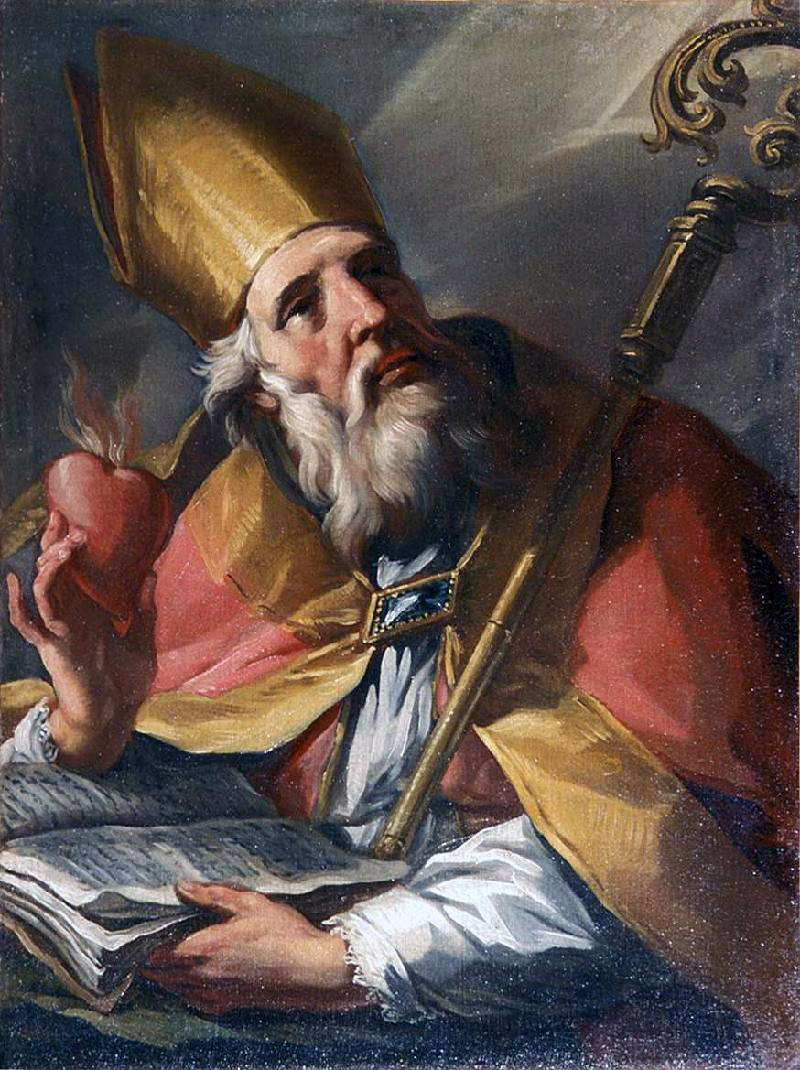
\includegraphics[width=0.5\textwidth]{ud-03/SanAgustin.jpg}
%\caption{San Agustín canonizado.\\
%(Fonte: wikimedia commons)}
%\label{fig:San-Agustin}
%\end{figure}

